\section{Ejercicio 1}
\subsection*{Instrucción}
Supongamos ahora que queremos definir una operación\par 
\texttt{numberOfRentalsWithDifferentOffices() : Integer} en la clase
\texttt{Customer} que devuelve el número de alquileres web que ha hecho un cliente self donde la oficina de recogida y de
entrega es diferente. En este momento del diseño del sistema todavía no sabemos qué estructura de datos
utilizaremos para guardar los alquileres que ha hecho/hace un cliente.

\subsection{Patrón de Diseño utilizado}
El objetivo de incorporar la nueva operación es introducir al sistema una forma de recuperar información específica acerca de alquileres web. 
Como todos los alquileres son realizados por clientes, necesitaríamos verificar cada uno y encontrar todos aquellos que cumplan que su alquiler 
además de ser mediante la página, cumplan que la oficina de recogida entrega sea diferente.\par
\vspace{0.15cm}
La descripción inicial del sistema no detalla que esta operación sea la única que hace falta o es la primera 
que se implementa referente a los alquileres. Es posible que en un futuro se necesite información de clientes que hayan hecho más de un alquiler 
o se necesite recuperar información de cuantas veces un coche ha sido alquilado.\par
\vspace{0.15cm}
Pensando en todos los casos que se puedan solicitar, es ineficiente simplemente hacer un bucle que recorra toda la colección y filtrar por 
la condición necesaria si el sistema puede escalar. Es por ello que el patrón \texttt{Iterador} es el más adecuado para implementar esta solución.\par
\vspace{0.15cm}
Este patrón de diseño nos permite acceder secuencialmente a los elementos de una colección, separando la lógica de iteración del \emph{cliente}\footnote{\textbf{¿Quiénes son los \emph{clientes}?} Este término no se refiere ni a las clases del sistema ni a los usuarios del programa, sino a las partes del código que utilizan el iterador para recorrer una colección. En este caso, el \emph{cliente} del iterador es el método \texttt{numberOfRentalsWithDifferentOffices()}.} y centralizándola 
en el propio iterador, sin mencionar que permite escalar con facilidad el sistema. Otra ventaja de usar esta patrón es que no expone la estructura interna 
de la colección y permite ser usada por varios \emph{clientes} simultáneamente.

\subsubsection*{Consideraciones}
Como estamos utilizando un \texttt{HashSet} para almacenar los alquileres, somos consientes que esta colección ya implementa el método \texttt{iterator()} de la 
interfaz \texttt{Iterable}. No sería correcto usar este iterator por las mismas razones recién comentadas; el iterador nativo de \texttt{HashSet} simplemente 
recorre los elementos uno por uno, sin ningún tipo de lógica adicional. Como queremos filtrar \texttt{Rentals} para recuperar los que cumplan una condición específica, 
tiene sentido implementar un iterador personalizado con este patrón que encapsule esa lógica en particular.

\newpage % Mostramos el diagrama en una nueva página

\subsection{Efectos sobre el Diagrama de Diseño}
\begin{figure}[H]
    \centering
     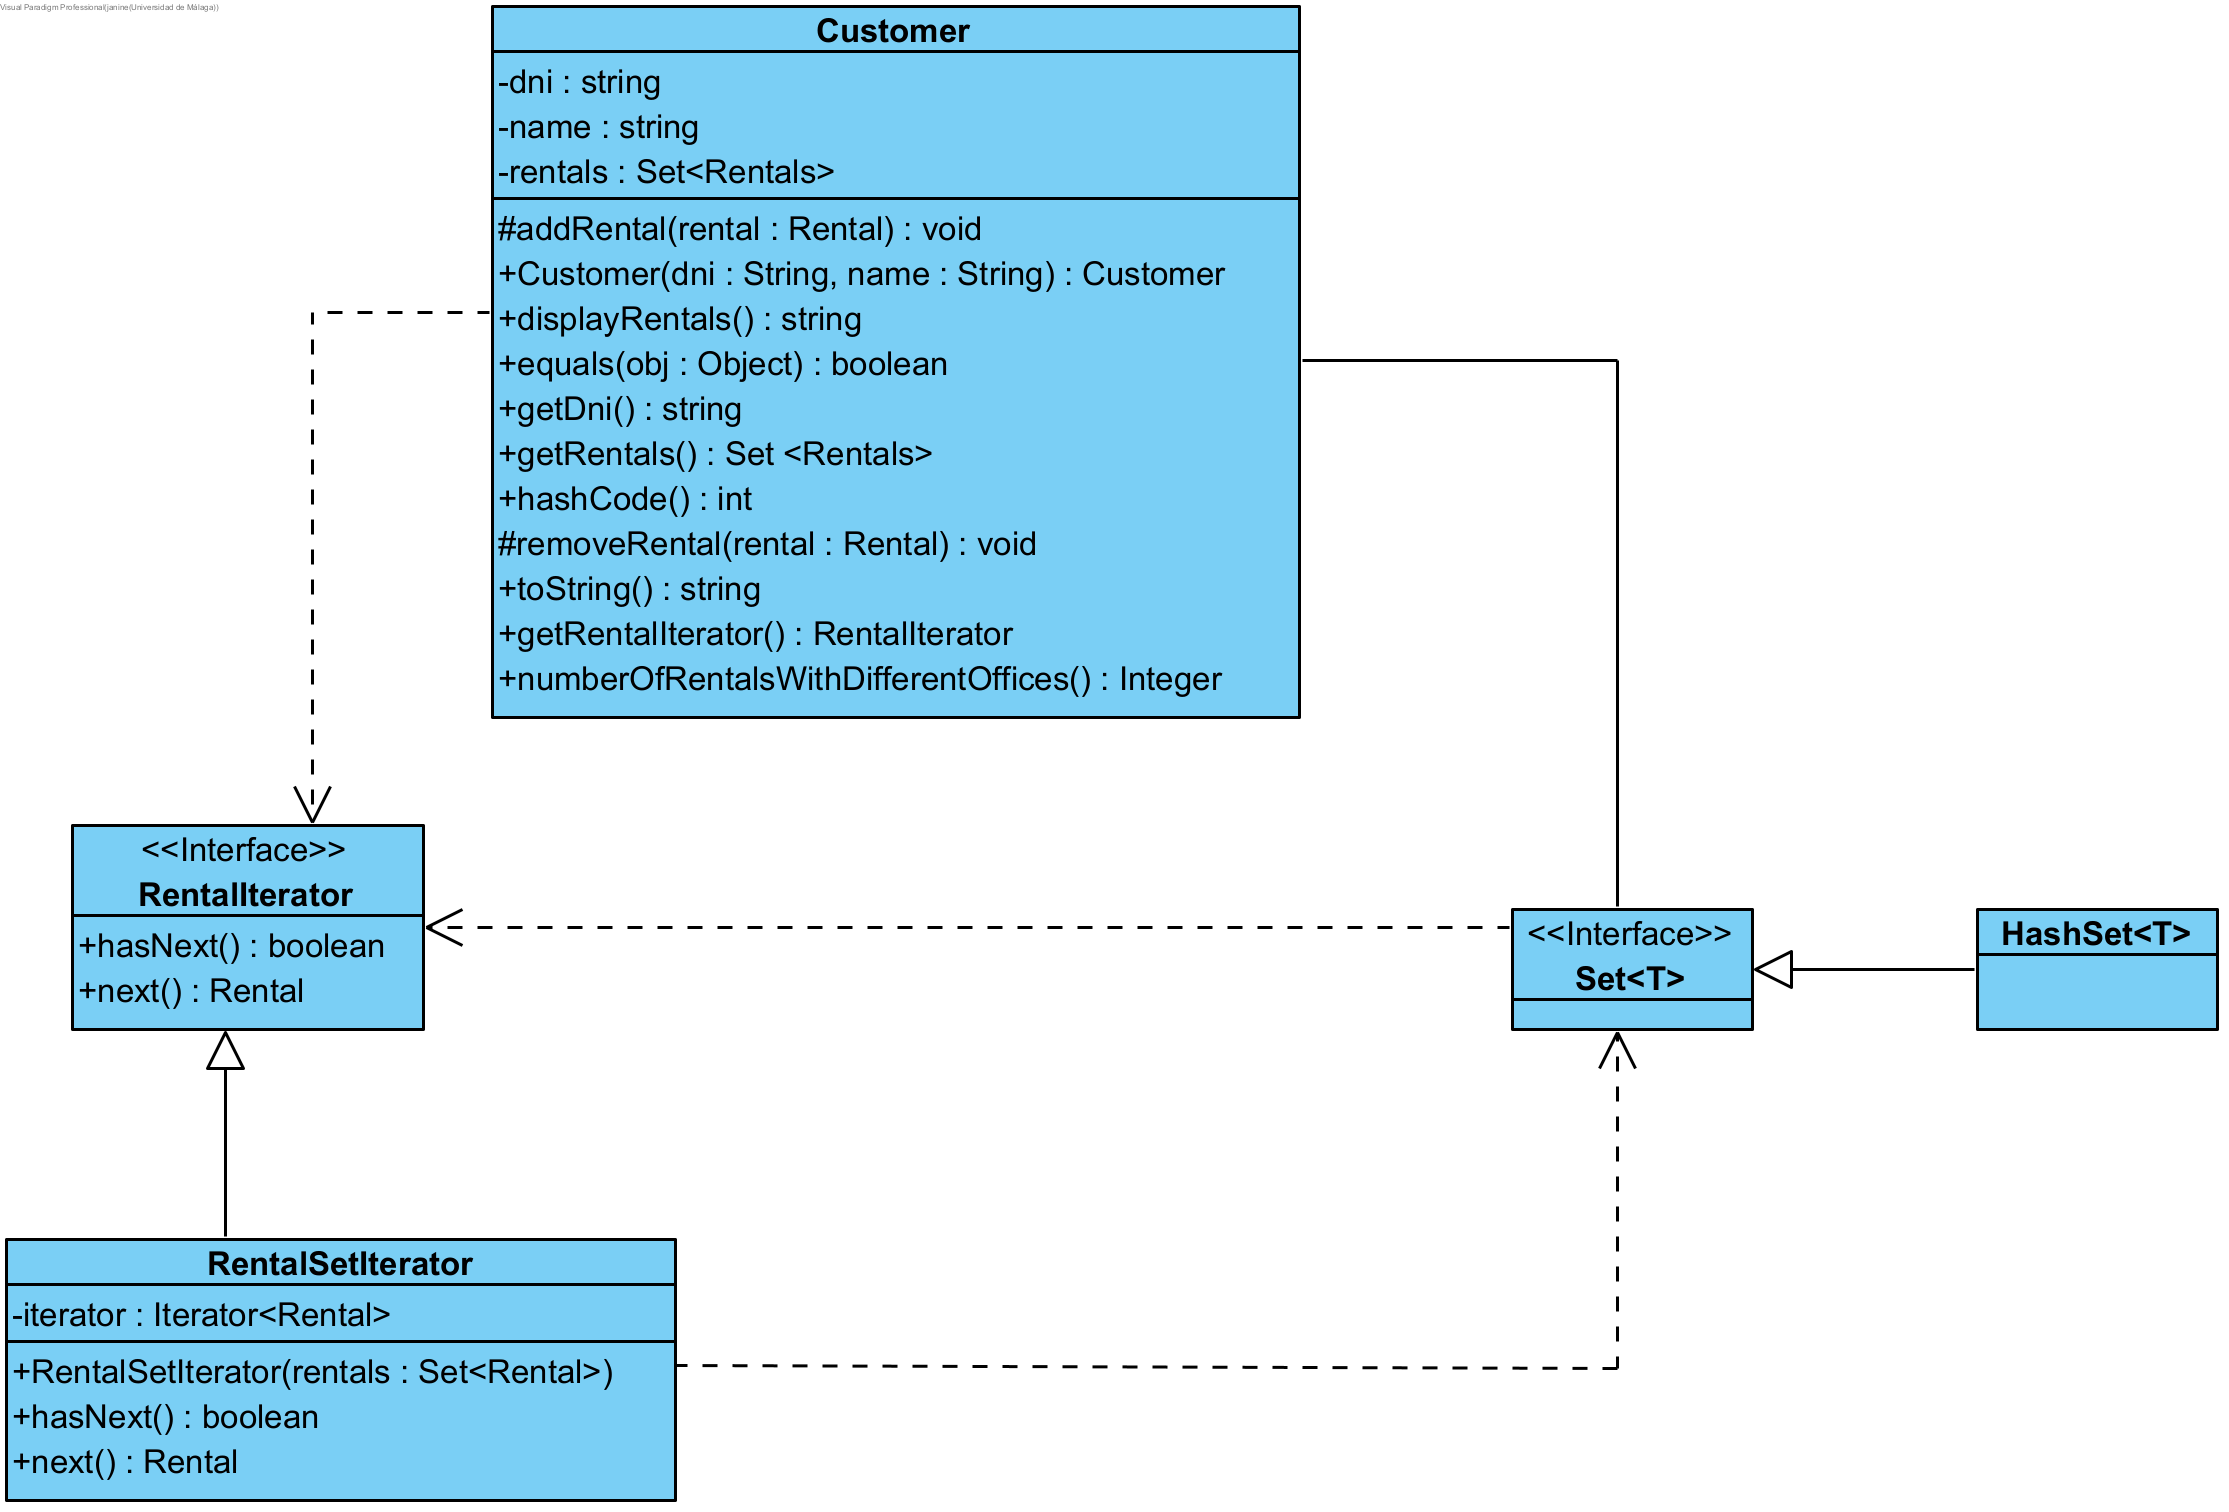
\includegraphics[width=0.70\linewidth]{assets/diagramas/UML_Apartado1.png}
     \caption{Diagrama de Diseño modificado para Ejercicio1}
\end{figure}
\vspace{0.50cm}
Hemos tenido que modificar el diseño original para poder implementar este patrón de diseño. Siguiendo la estructura presentada en los apuntes del Tema 6 en la página 108, tenemos:
\begin{itemize}
    \item \textbf{\texttt{Interfaz} RentalIterator:} Define las operaciones necesarias para recorrer la colección de elementos.
    \item \textbf{\texttt{Interfaz} RentalCollection:} Implementa las operaciones necesarias para crear una colección iterable. Es una \texttt{IterableCollection}.
    \item \textbf{\texttt{ConcreteCollection } RentalSet:} Almacena los elementos y devuelve un iterador para recorrerlos además de poder gestionarlos y recuperarlos.
    \item \textbf{\texttt{ConcreteIterator} RentalSetIterator:} Contiene la lógica específica para moverse de uno en uno a través de la colección.
    \item \textbf{\texttt{ConcreteIterator} FilteredRentalIterator:} Contiene la lógica que recorre solo los elementos de tipo \texttt{WebRental} cumpla con la condición de tener una oficina de recogida y entrega distintas.
\end{itemize}
\vspace{0.15cm}
Estructurar el diseño de esta manera, se alinea con el enunciado ya que estamos abstrayendo el tipo de colección usada para guardar los alquileres que ha hecho/hace un cliente.

\newpage % Mostramos la implementación en una nueva página

\subsection{Implementación de \textit{numberOfRentalsWithDifferentOffices():Integer}}
\begin{lstlisting}[style = javaNormal, language=Java] 

    introducir codigo aqui

\end{lstlisting} % Código en el documento "codigosEj1"

Sigue el patrón de diseño implementado ya que se ha modificado la clase para que este \emph{cliente} solo reciba el resultado del método 
sin exponer la lógica de la iteración. A continuación mostramos las operaciones que ocurren en segundo plano para devolver el resultado esperado del método.
\begin{enumerate}
    \item \emph{Cliente} (\texttt{Customer}) inicia el cálculo llamando al nuevo método.
    \item \texttt{RentalSet} crea el \texttt{FilteredRentalIterator} en respuesta.
    \item Este iterador, contiene la lógica filtrado para los elementos en la colección. Como se ve a continuación.
    \begin{lstlisting}[style = javaEspecifico, language=Java]
 // Clase FilteredRentalIterator
            [...]
    private void moveToNextValid() {
        nextRental = null;
        while (iterator.hasNext()) {
            Rental rental = iterator.next();
            if (rental instanceof WebRental) {
                WebRental webRental = (WebRental) rental;
                if (!webRental.getPickUpRentalOffice().equals(webRental.getDeliveryRentalOffice())) {
                    nextRental = rental;
                    break;
                }
            }
        }
    }
            [...]
\end{lstlisting}
    \item \emph{Cliente} utiliza el iterador para contar los elementos válidos.
    \item El cliente recibe el número total de alquileres que cumplen el filtro.
\end{enumerate}
\newpage

\newpage % Muestra el test

\subsection{Ejemplo de ejecución}
\begin{lstlisting}[style = javaNormal, language=Java] 
    // Crear cliente
    Customer customer2 = new Customer("87654321B", "Bob");
    // Crear modelos de coches
    Model modelA = new Model("Model A", 50);
    Model modelB = new Model("Model B", 70);
    // Crear oficinas de alquiler
    RentalOffice office1 = new RentalOffice("Office 1", 20);
    RentalOffice office2 = new RentalOffice("Office 2", 25);
    // Crear coches
    Car car1 = new Car("ABC-123", modelA, office1);
    Car car2 = new Car("XYZ-789", modelB, office2);
    // Crear fechas
    Date startDate1 = new GregorianCalendar(2024, Calendar.JANUARY, 1).getTime();
    Date endDate1 = new GregorianCalendar(2024, Calendar.JANUARY, 10).getTime();

    Date startDate2 = new GregorianCalendar(2024, Calendar.JANUARY, 5).getTime();
    Date endDate2 = new GregorianCalendar(2024, Calendar.JANUARY, 15).getTime();

    // Oficinas diferentes
    WebRental webRental1 = new WebRental(5, startDate1, endDate1, customer2, car1, office1);
    webRental1.setDeliveryRentalOffice(office2);

    // Oficinas iguales
    WebRental webRental2 = new WebRental(2, startDate1, endDate1, customer2, car2, office2);
    webRental2.setDeliveryRentalOffice(office2);

    // Usar nueva operacion implementada
    int rentalsWithDifferentOffices = customer2.numberOfRentalsWithDifferentOffices();

    System.out.println("Alquileres con oficinas diferentes: " + rentalsWithDifferentOffices);

    if (rentalsWithDifferentOffices == 1) {
        System.out.println("Correcto: El metodo devuelve el numero esperado.");
    } else {
        System.out.println("ERROR: El metodo devuelve un resultado incorrecto.");
    }
\end{lstlisting}


\subsubsection*{Output}

\begin{lstlisting}[style = javaNormal, language=Java] 
    [WebRental: Mon Jan 01 00:00:00 CET 2024 Wed Jan 10 00:00:00 CET 2024
    ; 2, WebRental: Mon Jan 01 00:00:00 CET 2024 Wed Jan 10 00:00:00 CET 2024
    ; 5]

    Alquileres con oficinas diferentes: 1
    Correcto: El metodo devuelve el numero esperado.
\end{lstlisting}

\vspace{1cm}

Los \texttt{toString()} usados para mostrar el Output fueron:


\begin{lstlisting}[style = javaEspecifico, language=Java] 
    // en Rental
    @Override
    public String toString() {
        return this.getClass().getName() + ": " + startDate + " " + endDate+"\n";
    }

    // en WebRental
    @Override
    public String toString() {
        return super.toString() + " ; " + deliveryTime.toString();
    }
\end{lstlisting}

